\section{Experimental results}\label{sec:experiments}
To save time, only the first, out of ten, trial is used to split out training data. For each category, one object is cut out for evaluation while the rest is used for training. Since the number of objects varies for every category, the number of training objects also differs.

By experiment, the accuracy for RGB channel is 54.80\%, for depth channel is 71.51\%, and for fusion is 63.66\%, as seen if Table \ref{tab:accuracy}. The results also show that the system is overfitting training data, as the accuracy on training set is approaching 100\%. 

A more detailed view of the results are illustrated as confusion matrices in Figure \ref{fig:rgb_confusion}, \ref{fig:dep_confusion}, and \ref{fig:fus_confusion}, with respect to the recognition results on color, depth, and fusion networks. For a confusion matrices $C$, the value at cell $C_{i,j}$ is equal to the number of observations known to be in group $i$ but predicted to be in group $j$. Therefore, the more values focusing on the diagonal the better it is since they are the correct recognition results ($i=j$). From confusion matrix figures, most of the results stays on the diagonal but there are several false recognition results on the two halves.

\begin{table}
	\centering
	\caption{Accuracy of the networks}
	\begin{tabular}{|c|c|c|c|}
		\hline 
		& Color & Depth & Fusion \\ 
		\hline 
		Training (top 1) & 98.48\% & 96.20\% & 100\% \\ 
		Evaluation (top 1) & 54.80\% & 71.51\% & 63.66\% \\ 
		Evaluation (top 5) & 76.91\% & 89.79\% & 85.63\% \\ 
		\hline 
	\end{tabular}
	\label{tab:accuracy} 
\end{table}


\begin{figure}
	\centering
	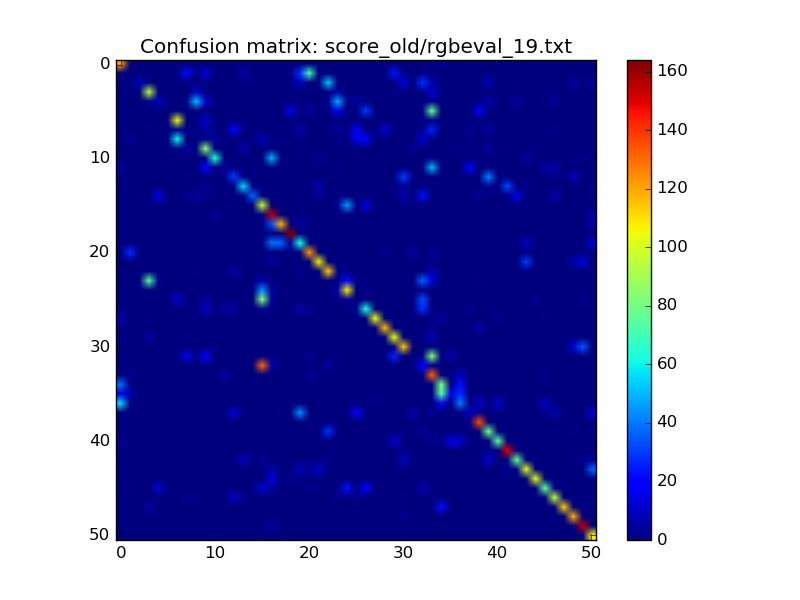
\includegraphics[trim={2cm 1cm 2.5cm 1.5cm}, clip, width=\linewidth]{images/rgb_t1_54_t5_77}
	\caption{Confusion matrix of RGB network.}
	\label{fig:rgb_confusion}
\end{figure}

\begin{figure}
	\centering
	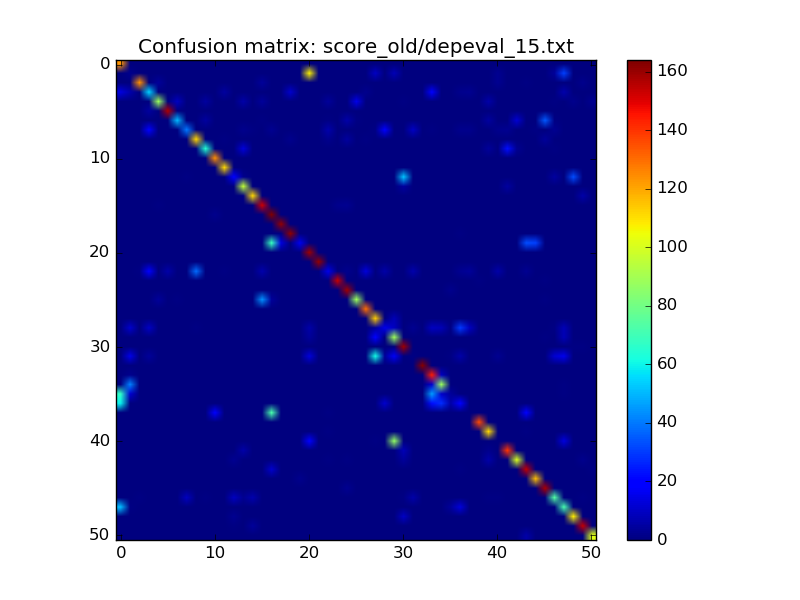
\includegraphics[trim={2cm 1cm 2.5cm 1.5cm}, clip, width=\linewidth]{images/dep_t1_71_t5_89}
	\caption{Confusion matrix of depth network.}
	\label{fig:dep_confusion}
\end{figure}

\begin{figure}
	\centering
	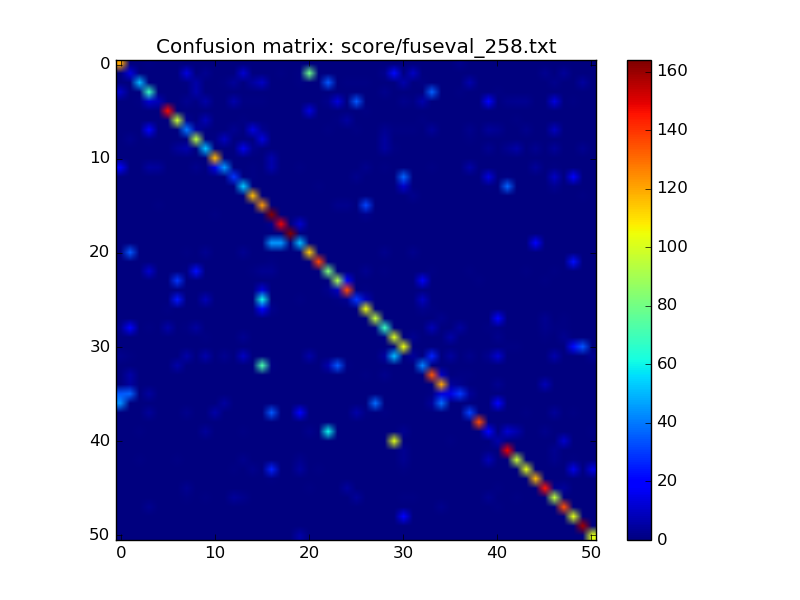
\includegraphics[trim={2cm 1cm 2.5cm 1.5cm}, clip, width=\linewidth]{images/fus_t1_63_t5_85}
	\caption{Confusion matrix of fusion network.}
	\label{fig:fus_confusion}
\end{figure}